\documentclass[12pt,halfline,a4paper,]{ouparticle}

% Packages I think are necessary for basic Rmarkdown functionality
\usepackage{hyperref}
\usepackage{graphicx}
\usepackage{listings}
\usepackage{color}
\usepackage{fancyvrb}
\usepackage{framed}

% For knitr::kable functionality
\usepackage{booktabs}
\usepackage{longtable}

%% To allow better options for figure placement
%\usepackage{float}

% Packages that are supposedly required by OUP sty file
\usepackage{amssymb, amsmath, geometry, amsfonts, verbatim, endnotes, setspace}

% For code highlighting I think
\DefineVerbatimEnvironment{Highlighting}{Verbatim}{commandchars=\\\{\}}
\definecolor{shadecolor}{RGB}{248,248,248}
\newenvironment{Shaded}{\begin{snugshade}}{\end{snugshade}}
\newcommand{\AlertTok}[1]{\textcolor[rgb]{0.94,0.16,0.16}{#1}}
\newcommand{\AnnotationTok}[1]{\textcolor[rgb]{0.56,0.35,0.01}{\textbf{\textit{#1}}}}
\newcommand{\AttributeTok}[1]{\textcolor[rgb]{0.77,0.63,0.00}{#1}}
\newcommand{\BaseNTok}[1]{\textcolor[rgb]{0.00,0.00,0.81}{#1}}
\newcommand{\BuiltInTok}[1]{#1}
\newcommand{\CharTok}[1]{\textcolor[rgb]{0.31,0.60,0.02}{#1}}
\newcommand{\CommentTok}[1]{\textcolor[rgb]{0.56,0.35,0.01}{\textit{#1}}}
\newcommand{\CommentVarTok}[1]{\textcolor[rgb]{0.56,0.35,0.01}{\textbf{\textit{#1}}}}
\newcommand{\ConstantTok}[1]{\textcolor[rgb]{0.00,0.00,0.00}{#1}}
\newcommand{\ControlFlowTok}[1]{\textcolor[rgb]{0.13,0.29,0.53}{\textbf{#1}}}
\newcommand{\DataTypeTok}[1]{\textcolor[rgb]{0.13,0.29,0.53}{#1}}
\newcommand{\DecValTok}[1]{\textcolor[rgb]{0.00,0.00,0.81}{#1}}
\newcommand{\DocumentationTok}[1]{\textcolor[rgb]{0.56,0.35,0.01}{\textbf{\textit{#1}}}}
\newcommand{\ErrorTok}[1]{\textcolor[rgb]{0.64,0.00,0.00}{\textbf{#1}}}
\newcommand{\ExtensionTok}[1]{#1}
\newcommand{\FloatTok}[1]{\textcolor[rgb]{0.00,0.00,0.81}{#1}}
\newcommand{\FunctionTok}[1]{\textcolor[rgb]{0.00,0.00,0.00}{#1}}
\newcommand{\ImportTok}[1]{#1}
\newcommand{\InformationTok}[1]{\textcolor[rgb]{0.56,0.35,0.01}{\textbf{\textit{#1}}}}
\newcommand{\KeywordTok}[1]{\textcolor[rgb]{0.13,0.29,0.53}{\textbf{#1}}}
\newcommand{\NormalTok}[1]{#1}
\newcommand{\OperatorTok}[1]{\textcolor[rgb]{0.81,0.36,0.00}{\textbf{#1}}}
\newcommand{\OtherTok}[1]{\textcolor[rgb]{0.56,0.35,0.01}{#1}}
\newcommand{\PreprocessorTok}[1]{\textcolor[rgb]{0.56,0.35,0.01}{\textit{#1}}}
\newcommand{\RegionMarkerTok}[1]{#1}
\newcommand{\SpecialCharTok}[1]{\textcolor[rgb]{0.00,0.00,0.00}{#1}}
\newcommand{\SpecialStringTok}[1]{\textcolor[rgb]{0.31,0.60,0.02}{#1}}
\newcommand{\StringTok}[1]{\textcolor[rgb]{0.31,0.60,0.02}{#1}}
\newcommand{\VariableTok}[1]{\textcolor[rgb]{0.00,0.00,0.00}{#1}}
\newcommand{\VerbatimStringTok}[1]{\textcolor[rgb]{0.31,0.60,0.02}{#1}}
\newcommand{\WarningTok}[1]{\textcolor[rgb]{0.56,0.35,0.01}{\textbf{\textit{#1}}}}

% For making Rmarkdown lists
\providecommand{\tightlist}{%
  \setlength{\itemsep}{0pt}\setlength{\parskip}{0pt}}

% Part for setting citation format package: natbib

% Part for setting citation format package: biblatex

% Part for indenting CSL refs

% Pandoc header

\begin{document}

\title{Measuring the Relationship Between National Economies and Confidence in
Economic Institutions}

\author{%
\name{Author Bruno Guimaraes Ubiali}\address{Department of Anthropology, University of Georgia}
\and
\name{Zachary Thomas McDowell}\address{Department of Political Science, University of Georgia}\thanks{Corresponding author; Email: \href{mailto:}{}}
}

\abstract{People's opinions on economic institutions can vary according to the
level of development of their countries of residence, which has
implications for levels of investment in national and international
markets. This paper aims at testing the hypothesis that people who
reside in developed countries have a higher level of trust in economic
institutions than people who reside in developing countries. We draw on
secondary data from the World Values Survey (WVS) for the United States,
Mexico, and Chile. For data analyses, we used the software R for
producing graphs and statistical inferences. The results do not confirm
our hypothesis; there is no homogeneous patter of response according to
the level of economic development of the country. The results indicate
that people in Mexico have higher confidence in banks than US and Chile
inhabitants}

\date{\today}

\keywords{OECD; Economics; Development; IMF}

\maketitle



\hypertarget{introduction}{%
\section{Introduction}\label{introduction}}

People's opinions on economic institutions can vary according to the
level of development of their countries of residence. This has
implications for trust in economic policies, which can in turn influence
levels of investment in national and international markets. Based on
this, we hypothesized that people who reside in developed countries have
a higher level of trust in economic institutions than people who reside
in developing countries. This paper aims at testing this hypothesis,
drawing on the World Values Survey (WVS), which takes a global approach
to inquiry people about their cultural values as well as attitudes and
perceptions regarding multilateral institutions, economy, education,
health, among many others (ref). We used specifically the question of
confidence at the International Monetary Fund (IMF), and institution
created in the United States in the 1940s with the main objective of
promoting international financial stability and economic cooperation
(ref). We purposefully selected answers from three countries that
reflect a range of development levels in the Americas: United States,
Mexico, and Chile.

\hypertarget{materials-and-methods}{%
\section{Materials and Methods}\label{materials-and-methods}}

For our research purposes, we decided to examine the various responses
found in the World Values Survey Wave 7 (2017-2020). Originally, the
goal was to compare the results from the top three and bottom three
countries in the Organization for Economic Co-operation and Development
(OECD) concerning GDP per capita. Unfortunately, some of the countries
that ranked at or near the top of the OECD list did not record responses
for the survey questions that were selected to measure economic
attitudes (Luxembourg, Ireland, Norway, Switzerland). As a result, our
study limits its analysis to the following three countries: Chile,
Mexico, and the United States.

Cross referencing the World Values Survey data with the data gathered by
the OECD, we established that Chile and Mexico were the two countries
that fulfilled the needs of the study; they countries ranked near the
bottom of the OECD in terms of GDP per capita and gave responses to the
survey questions that were chosen to measure economic attitudes.

On the other side of the spectrum, the United States (U.S.) was the
highest ranking country in the OECD that also responded to the
aforementioned questions that were picked for this paper. Additionally,
the U.S. is a uniquely well situated country to serve as the foil for
Chile and Mexico, due to the the U.S. having one of the largest national
economies in the world (NEED CITE). Subsequently, it will be interesting
to see how the two poorer countries (Chile and Mexico) compare to the
U.S., with the assumption that people associate financial and economic
insititutions with economic outcomes and conditions (POSSIBLE CITE
NEEDED).

```fig7 \textless- ggplot(data = OECD.df) + geom\_col(mapping = aes(x =
LOCATION, y = VALUE)) + labs(title = ``OECD Countries GDP per capita'',
x = ``Countries'', y = ``USD (Thousands)'') + theme\_gray()

An equation with a label for cross-referencing:

\begin{equation}\label{eq:eq1}
\int^{r_2}_0 F(r,\varphi){\rm d}r\,{\rm d}\varphi = [\sigma r_2/(2\mu_0)]
\int^{\infty}_0\exp(-\lambda|z_j-z_i|)\lambda^{-1}J_1 (\lambda r_2)J_0
(\lambda r_i\,\lambda {\rm d}\lambda)
\end{equation}

This equation can be referenced as follows: Eq. \ref{eq:eq1}

\hypertarget{hypotheses}{%
\subsection{Hypotheses}\label{hypotheses}}

A numbered list:

\begin{enumerate}
\def\labelenumi{\arabic{enumi})}
\tightlist
\item
  People that live in lower GDP per capita countries will harbor
  negative attitudes towards various financial and/or economic
  institutions.
\item
  SPeople that live in higher GPD per capita countries will harbor
  positive attitudes towards various financial and/or economic
  institutions.
\end{enumerate}

\hypertarget{results}{%
\section{Results}\label{results}}

\hypertarget{generate-a-figure.}{%
\subsection{Generate a figure.}\label{generate-a-figure.}}

You can reference this figure as follows: Fig. \ref{fig:fig1}.

\begin{Shaded}
\begin{Highlighting}[]
\KeywordTok{plot}\NormalTok{(}\DecValTok{1}\OperatorTok{:}\DecValTok{5}\NormalTok{,}\DataTypeTok{pch=}\DecValTok{19}\NormalTok{,}\DataTypeTok{main=}\StringTok{"Some data"}\NormalTok{,}\DataTypeTok{xlab=}\StringTok{"Distance (cm)"}\NormalTok{,}\DataTypeTok{ylab=}\StringTok{"Time (hours)"}\NormalTok{)}
\end{Highlighting}
\end{Shaded}

\begin{figure}[p]
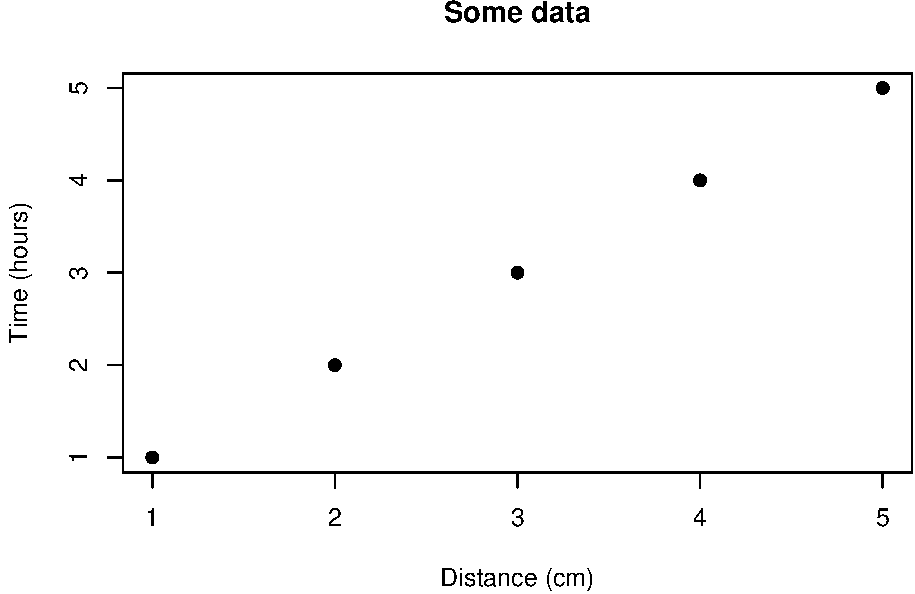
\includegraphics[width=1\linewidth]{Markdown-v3.1_files/figure-latex/fig2-1} \caption{This is the second figure.}\label{fig:fig2}
\end{figure}

Reference to second figure: Fig. \ref{fig:fig2}

\begin{verbatim}

You can reference this table as follows: Table \ref{tab:tab1}.

## Generate a table using `kable`


```r
df = data.frame(ID=1:3,code=letters[1:3])

# kable can alse be used for creating tables
knitr::kable(df,caption="This is the table caption",format="latex",
             booktabs=TRUE,label="tab2")
\end{verbatim}

\begin{table}

\caption{\label{tab:tab2}This is the table caption}
\centering
\begin{tabular}[t]{rl}
\toprule
ID & code\\
\midrule
1 & a\\
2 & b\\
3 & c\\
\bottomrule
\end{tabular}
\end{table}

You can reference this table as follows: Table \ref{tab:tab2}.

\hypertarget{discussion}{%
\section{Discussion}\label{discussion}}

You can cross-reference sections and subsections as follows: Section
\ref{materials-and-methods} and Section \ref{a-subsection}.

\textbf{\emph{Note:}} the last section in the document will be used as
the section title for the bibliography.

\hypertarget{references}{%
\section{References}\label{references}}






\end{document}
